\begin{figure}[!htbp]
  \centering
  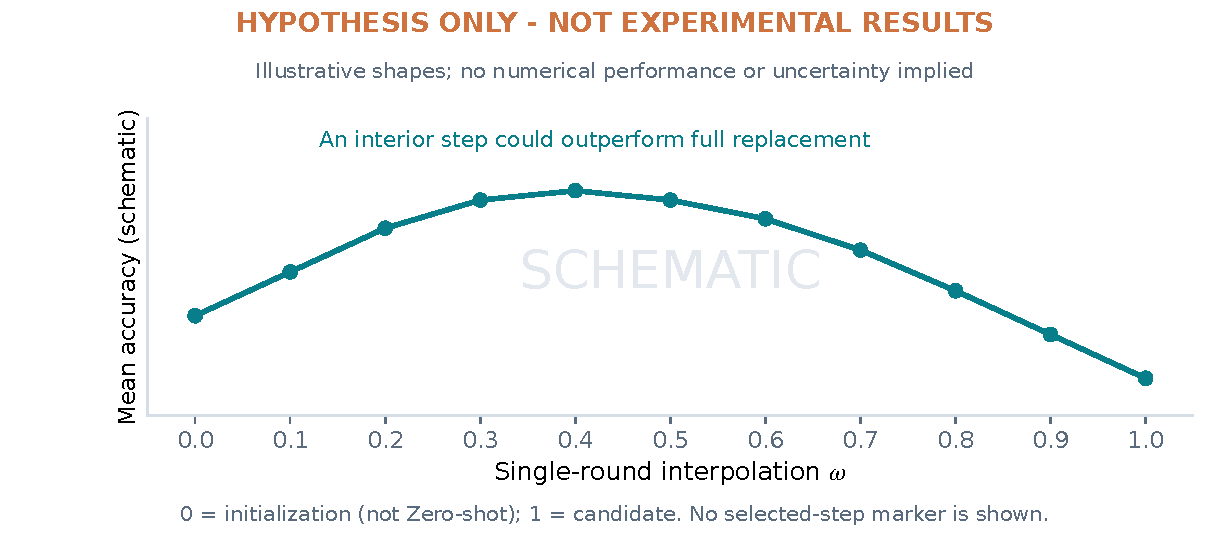
\includegraphics[width=0.78\linewidth]{figures/hypothesis_step_accuracy.pdf}
  \caption{\textbf{单轮步长--准确率的预期趋势示意，非实验结果。}可能的情形是中间步长优于完整替换；示意峰值不对应推荐步长。$\omega=0$ 为初始化模型而非 Zero-shot，$\omega=1$ 为完整候选更新。图中没有实际选步标记。}
  \label{fig:ink-step-size-analysis}
\end{figure}
